\documentclass[12pt]{article}
\usepackage{light}

\hidesolutions
%\showsolutions

\newcommand{\edge}[2]{#1\text{---}#2}
\newcommand{\mfigure}[3]{\bigskip\centerline{\resizebox{#1}{#2}{\includegraphics{#3}}}\bigskip}

\begin{document}

\recitation{8}{October 7, 2016}

%%%%%%%%%%%%%%%%%%%%%%%%%%%%%%%%%%%%%%%%%%%%%%%%%%%%%%%%%%%%%%%%%%%%%%%%%%%%%%%
\section*{Routing in a Bene\u{s} Network}

In lecture, we saw that the Bene\u{s} network has a max congestion of
1; that is, every permutation can be routed in such a way that a
single packet passes through each switch.  Let's work through an
example.  A Bene\u{s} network of size $N = 8$ is attached.

\begin{enumerate}
\item Within the Bene\u{s} network of size $N = 8$, there are two
subnetworks of size $N = 4$.  Put boxes around these.  Hereafter,
we'll refer to these as the \textit{upper} and \textit{lower}
subnetworks.

\solution{
\ \\
\mfigure{!}{2in}{benes-decomp}
}

\item Now consider the following permutation routing problem:
%
\begin{align*}
\pi(0) & = 3 & \pi(4) & = 2 \\
\pi(1) & = 1 & \pi(5) & = 0 \\
\pi(2) & = 6 & \pi(6) & = 7 \\
\pi(3) & = 5 & \pi(7) & = 4
\end{align*}
%
Each packet must be routed through either the upper subnetwork or the
lower subnetwork.  Construct a graph with vertices 0, 1, \ldots, 7 and
draw a \textit{dashed} edge between each pair of packets that can not
go through the same subnetwork because a collision would occur in the
second column of switches.

\solution{
\ \\
\mfigure{!}{2in}{rec-const1}
}

\item Add a \textit{solid} edge in your graph between each pair of
packets that can not go through the same subnetwork because a
collision would occur in the next-to-last column of switches.

\solution{
\ \\
\mfigure{!}{2in}{rec-const2}
}

\item Color (i.e., label) the vertices of your graph red and blue so
  that adjacent vertices get different colors.  Why must this be
  possible, regardless of the permutation $\pi$?

\solution{This must be possible, because the dashed edges form a
matching and the solid edges form another matching.  Because of the
result you proved in homework, when you combine the edges, the result
is a bipartite graph, which must be 2-colorable.
%
%This must be possible, because edges in a cycle are
%alternately dashed and solid.  Thus, every cycle has even length,
%which implies that the graph is bipartite or, equivalently,
%2-colorable.

\mfigure{!}{2in}{rec-const3}
}

\item Suppose that red vertices correspond to packets routed through
the upper subnetwork and blue vertices correspond to packets routed
through the lower subnetwork.  On the attached copy of the Bene\u{s}
network, highlight the first and last edge traversed by each packet.

\solution{
\ \\
\mfigure{!}{3in}{rec-benes1}
}

\item All that remains is to route packets through the upper and
lower subnetworks.  One way to do this is by applying the procedure
described above recursively on each subnetwork.  However, since the
remaining problems are small, see if you can complete all the paths 
on your own.

\solution{
\ \\
\mfigure{!}{3in}{rec-benes2}
}

\end{enumerate}

\instatements{\newpage}

\rotatebox{90}{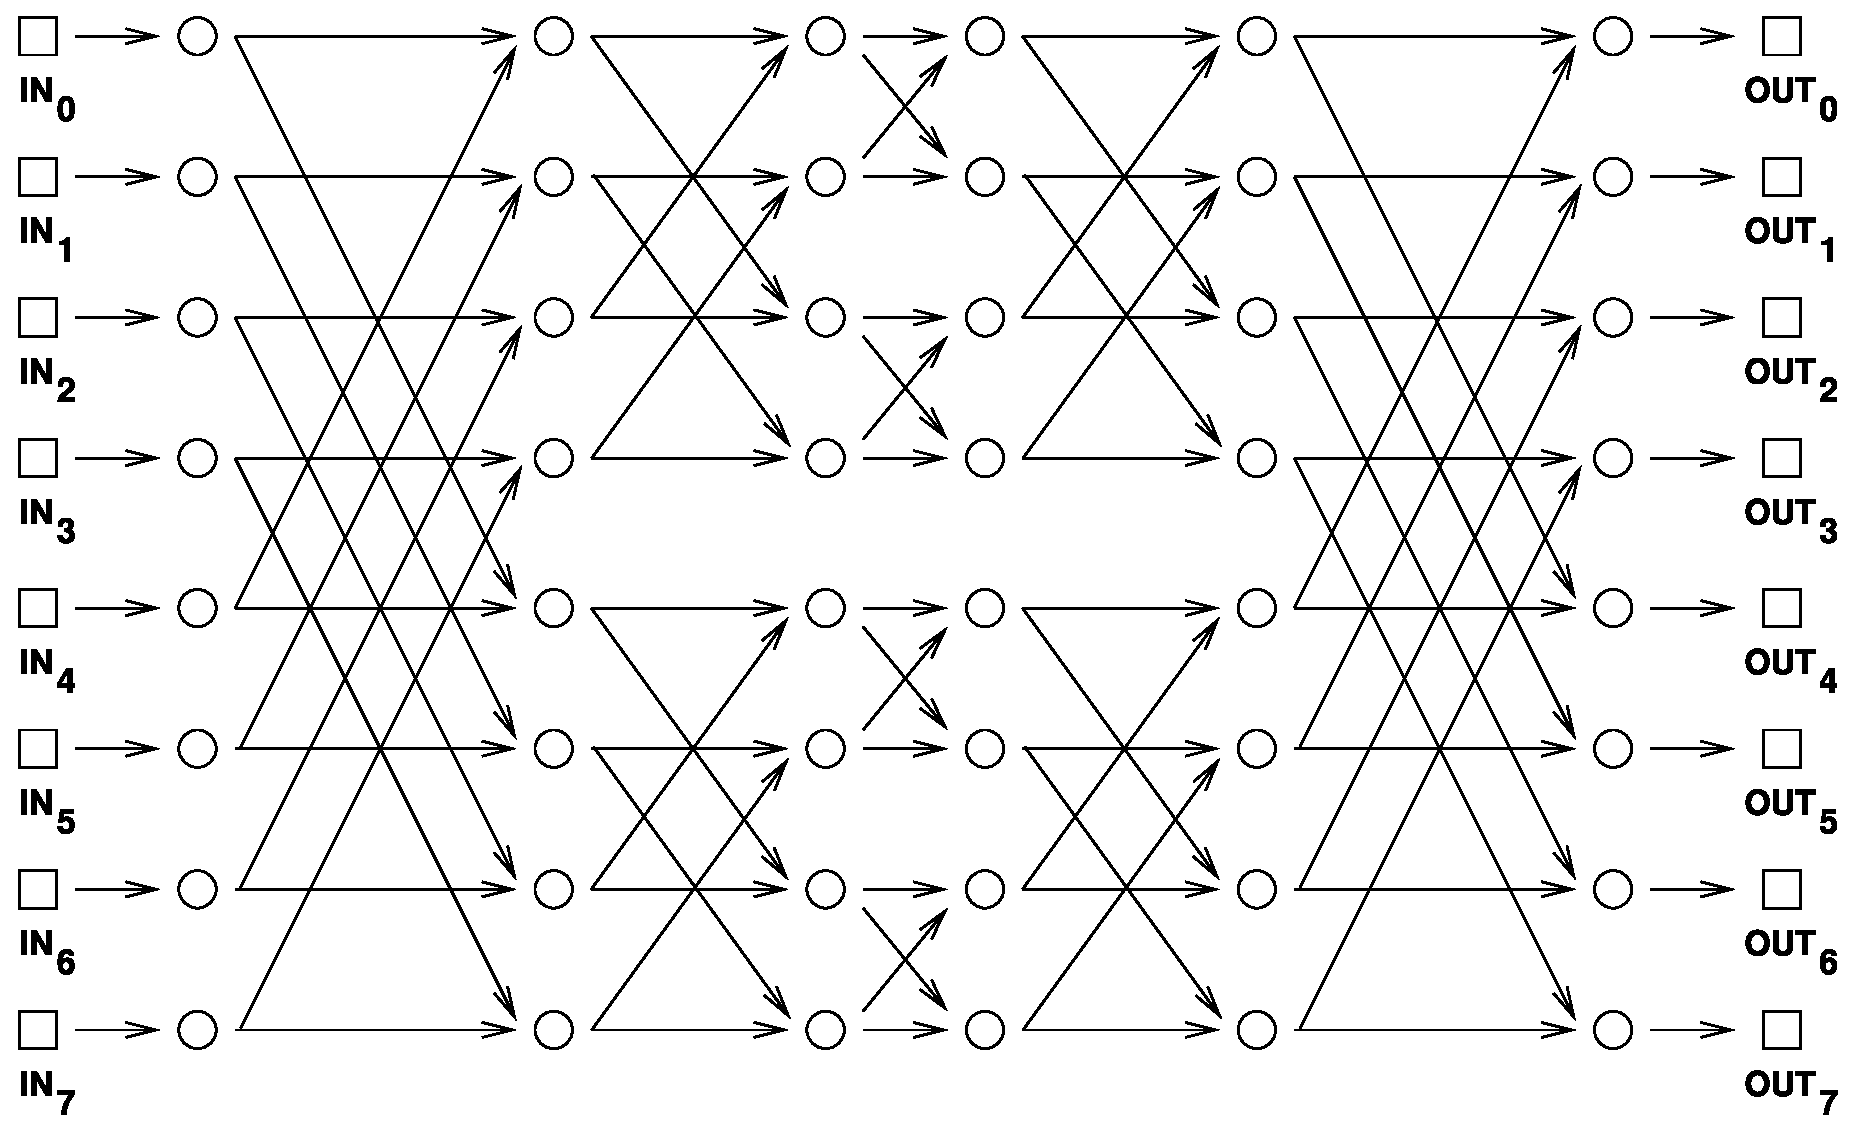
\includegraphics
[width=8.25in]{benes}}

\section{Euler tours}

\begin{enumerate}[(a)]
    \item Prove that a graph $G$ has an Euler tour if and only if: i) every vertex of $G$ has even degree, and ii) the subgraph obtained after removing all isolated vertices is connected. (An \emph{isolated vertex} is a vertex of degree $0$.)

Note that there are two directions to prove!

\solution{
    Let $G'$ be the subgraph induced by the vertices that are not isolated vertices. Note that $G'$ has an Euler tour if and only if $G$ has. 
    Any Euler tour must visit every vertex in $G'$, since all edges must be visited. 
    Thus ii) is certainly a necessary condition for the existence of an Euler tour.

    The rest of the proof is as in the proof of Theorem 5.6.3 in the book (pp.~159--160).
}
\item Come up with a necessary and sufficient condition for the existence of an Euler tour in a \emph{directed} graph. Adapt your proof above to prove that your condition is the right one.
    %Adapt your proof above to show that in a directed graph, an Eulerian circuit exists if and only if for every vertex, the indegree equals the outdegree.
%\emph{(Once you've figured out the condition, you might want to skip writing down the proof until you've done the rest of the recitation.)}

    \solution{The condition is: an Euler tour exists if and only if i) for every vertex, the indegree equals the outdegree, and ii) the subgraph obtained after removing all isolated vertices is strongly connected.

        The proof is basically the same. 
        Again, let $G'$ be the subgraph of $G$ induced on the non-isolated vertices of $G$; $G'$ has an Euler tour if and only if $G$ does.
        Any Euler tour provides a directed path between any two vertices of $G'$ (since we need to visit every arc), and must enter and exit a vertex the same number of times; so the condition is certainly necessary. 
        
        Now suppose the condition holds, and let $W = w_0, w_1, \ldots, w_k$ be a longest walk in $G'$ using every directed edge at most once. 
        Then $W$ must be a closed walk; for suppose that $w_k \neq w_0$. Then we must have entered $w_k$ one more time than we left it, which means that there is some outgoing directed edge that we have not used. This would allow us to extend the walk, contradicting that $W$ was as long as possible.

        Suppose that $W$ is not an Euler tour. 
        There must be an unused edge directed away from some vertex in the walk $W$; for if not, there would be no path from any vertex on $W$ to a vertex not in $W$, contradicting the assumption that $G'$ is strongly connected.  
        Let $w_i \to u$ be this edge. Construct a walk $W'$ beginning with this edge and traversing only unused edges, stopping when we cannot make a move. Again by the condition that indegree equals outdegree, this walk will end at $w_i$. We thus obtain a longer walk 
        \[ W' = w_0, w_1, \ldots, w_i, u, \ldots, w_i, w_{i+1}, \ldots, w_k. \]
        This is again a contradiction.

    }

%    \begin{comment}
%\item Based on your proof of b), give an algorithm to find an Euler tour, when one exists, in the directed case. % Your algorithm should be reasonably efficient.
%
%    \solution{
%        
%        \begin{enumerate}
%            \item Let $W = v_0$, where $v_0$ be an arbitrary vertex. Let $E' = E$.
%            \item Repeat until $E'$ is empty
%                \begin{enumerate}
%                    \item Choose any vertex $v_i$ in the walk $W$ that is adjacent to some edge in $E'$
%                    \item Do a walk $W' = v_i, w_1, w_2, \ldots, w_k$ in $G'=(V, E')$ that starts at $v_i$ and that uses each edge at most once, until no steps are possible. This walk will end at $w_k = v_i$.
%                        Remove all edges of this walk from $E'$.
%                        Replace $W = v_0, v_1, \ldots, v_i, \ldots, v_k$ with the walk
%                        \[ v_0, \ldots, v_i, w_1, \ldots, w_{k-1}, v_i, \ldots, v_k. \]
%                \end{enumerate}
%        \end{enumerate}
%    } 
%\end{comment}
%
%        Choose an arbitrary vertex $v_0$, and begin walking from this node, at each step choosing an arbitrary outgoing directed edge. 
%        Once an edge is traversed, remove it from the graph (burn your bridges so to speak).
%        Eventually, this walk gets stuck; say we get the walk $v_0, v_1, \ldots, v_k$. 
%        Since we're stuck, and indegree is equal to outdegree at all vertices, it must be that $v_k = v_0$. So we have a closed walk.
%
%        
%        If there are any remaining edges, we will extend our walk.
%        Let $W = v_0, v_1, \ldots, v_k=v_0$ be the closed walk we have so far, and let $v_i$ be any node which touches some remaining edges. 
%        (Note that if we have used every edge that touches a node in the walk, we must have used all edges, since the graph is connected.)
%        Then do a walk $v_i, w_1, w_2, \ldots, w_r$ of unused edges starting from $v_i$. Again, this must stop at $v_i$. We can thus splice this together with $W$ to obtain a longer closed walk
%        \[ v_0, v_1, \ldots, v_i, w_1, w_2, \ldots, w_{r-1}, v_i, v_{i+1}, \ldots, v_k. \]
%        We continue this process, each time getting a longer walk, until we've exhausted all the edges. 
%    }

\end{enumerate}

%%%%%%%%%%%%%%%%%%%%%%%%%%%%%%%%%%%%%%%%%%%%%%%%%%%%%%%%%%%%%%%%%%%%%%%%%%%%%%%

\end{document}
